\documentclass[11pt, A4paper,norsk]{article}
\usepackage[utf8]{inputenc}
\usepackage[T1]{fontenc}
\usepackage{babel}
\usepackage{amsmath}
\usepackage{amsfonts}
\usepackage{amsthm}
\usepackage[colorlinks]{hyperref}
\usepackage{listings}
\usepackage{color}
\usepackage{hyperref}
\usepackage{graphicx}
\usepackage{cite}

\definecolor{dkgreen}{rgb}{0,0.6,0}
\definecolor{gray}{rgb}{0.5,0.5,0.5}
\definecolor{daynineyellow}{rgb}{1.0,0.655,0.102}
\definecolor{url}{rgb}{0.1,0.1,0.4}

\lstset{frame=tb,
	language=Python,
	aboveskip=3mm,
	belowskip=3mm,
	showstringspaces=false,
	columns=flexible,
	basicstyle={\small\ttfamily},
	numbers=none,
	numberstyle=\tiny\color{gray},
	keywordstyle=\color{blue},
	commentstyle=\color{daynineyellow},
	stringstyle=\color{dkgreen},
	breaklines=true,
	breakatwhitespace=true,
	tabsize=3
}

\lstset{inputpath="C:/Users/Torstein/Documents/UiO/Fys-mek1110/Python programmer"}
\hypersetup{colorlinks, urlcolor=url}

\author{Torstein Solheim Ølberg}
\title{Svar på Oblig nr. i Fys-Mek1110}







\begin{document}
\maketitle
	\begin{center}
\Large \textbf{Oppgaver}
	\end{center}









		\paragraph{a)}
			\begin{flushleft}
Find the velocity of the center of mass for the system before the collision. \\
\vspace{1mm}
\textbf{Løsning:}
\vspace{1mm}
				\begin{align}
\vec{R} = \frac{1}{M} \sum_{i} m_i \vec{r_i} \nonumber \\
\vec{R} = \frac{1}{M}(mr + mr) = \frac{1}{2m} \cdot m r_1 \nonumber \\
\vec{V} = \frac{\partial}{\partial t} \vec{R} = \frac{\partial \frac{\vec{r}}{2}}{\partial t} = \frac{1}{2} \frac{\partial \vec{r}}{\partial t} = \frac{1}{2} v_0 \nonumber
				\end{align}
			\end{flushleft}










		\paragraph{b)}
			\begin{flushleft}
Find the velocity of the center of mass of the system after the collision. \\
\vspace{1mm}
\textbf{Løsning:}
\vspace{1mm}
				\begin{align}
p_0 = p_1 \nonumber \\
v_0 = 2mv_1 \Rightarrow v_1 = \frac{v_0}{2} \nonumber
				\end{align}
			\end{flushleft}









		\paragraph{c)}
			\begin{flushleft}
What is the change in the system's kinetic energy through the collision. \\
\vspace{1mm}
\textbf{Løsning:} \\
\vspace{1mm}
				\begin{align}
E_k = \frac{1}{2}Mv^2 \nonumber \\
E_{k,0} = 2 \cdot \frac{1}{2} m(\frac{1}{2}v_0)^2 + \frac{1}{2} \cdot 2m(\frac{1}{2}v_0)^2 = \frac{1}{2}mv_0^2 \nonumber \\
E_{k,1} = \frac{1}{2} \cdot 2m(\frac{1}{2}v_0)^2 = \frac{1}{4}mv_0^2 \nonumber \\
E_[k,1] - E_{k,0} = \frac{1}{4}mv_0^2 - \frac{1}{2}mv_0^2 = - \frac{1}{4}mv_0^2 \nonumber 
				\end{align}
			\end{flushleft}









		\paragraph{d)}
			\begin{flushleft}
What is the velcoity of the center of mass immediately after the atoms are attached with the spring, that is, when atom $A$ is at the distance $b$ from atom $B$? What is the change in kinetic energy for the system before and immediately after the collision? \\
\vspace{1mm}
\textbf{Løsning:} \\
\vspace{1mm}
				\begin{align}
\vec{R} = \frac{1}{M}mb = \frac{1}{2m}mb = \frac{b}{2} \nonumber \\
\vec{V} = \frac{v_0}{2} \nonumber \\
E_{k,0} = E_{k,1} \nonumber
				\end{align}
Kinetisk energi til systemet før og etter kollisjon er like fordi støt med fjær er elastisk.
			\end{flushleft}











		\paragraph{e)}
			\begin{flushleft}
Show that the force on atom $A$ is: $F = k((x_B - x_A) - b)$, and find a corresponding expression for the force on atom $B$. \\
\vspace{1mm}
\textbf{Løsning:} \\
\vspace{1mm}
				\begin{align}
F_A = k \Delta x = k((x_A - x_B) - b) \nonumber \\
F_B = - k((x_B - x_A) - b) \nonumber
				\end{align}
Der delta x er endringen i lengden på fjæra som vil være avstanden mellom de to kulene minus ekvilibrium.
			\end{flushleft}









		\paragraph{f)}
			\begin{flushleft}
Find expressions for the acceleration for atom $A$ and $B$, and formulate the differential equations you need to solve to find the motion of the atoms, including the initial conditions. \\
\vspace{1mm}
\textbf{Løsning:} \\
\vspace{1mm}
				\begin{align}
ma_A = k(x_B - x_A - b) \Rightarrow a_A = \frac{k(x_B - x_A - b)}{m} \nonumber \\
a_B = - \frac{k(x_B - x_A - b)}{m} \nonumber \\
x_{A,n}'' = \frac{k(x_{b,n} - x_{A,n} - b)}{m} \nonumber \\
x_{A,n+1}' = x_{A,n} + x_{A,n}'' \cdot dt \nonumber \\
x_{A,n+1} = x_{A,n} + x_{A,n}' \cdot dt \nonumber \\
x_{B,n}'' = - \frac{k(x_{b,n} - x_{A,n} - b)}{m} \nonumber \\
x_{B,n+1}' = x_{B,n} + x_{B,n}'' \cdot dt \nonumber \\
x_{B,n+1} = x_{B,n} + x_{B,n}' \cdot dt \nonumber
				\end{align}
			\end{flushleft}









		\paragraph{g)}
			\begin{flushleft}
Write a program to determine the positions and velocities of atom $A$ and atom $B$ as a function of time. Assume $m = 0.1$, $k = 20$, $b = 0.2$, $v_0 = 1.0$, and $\Delta t = 0.001$. \\
\vspace{1mm}
\textbf{Løsning:} \\
\vspace{1mm}
\lstinputlisting{oblig6_g.py}
			\end{flushleft}









		\paragraph{h)}
			\begin{flushleft}
Plot the position as a function of time for the center of mass of the system and for each of the atoms. \\
\vspace{1mm}
\textbf{Løsning:} \\
\vspace{1mm}
\lstinputlisting{oblig6_h.py}
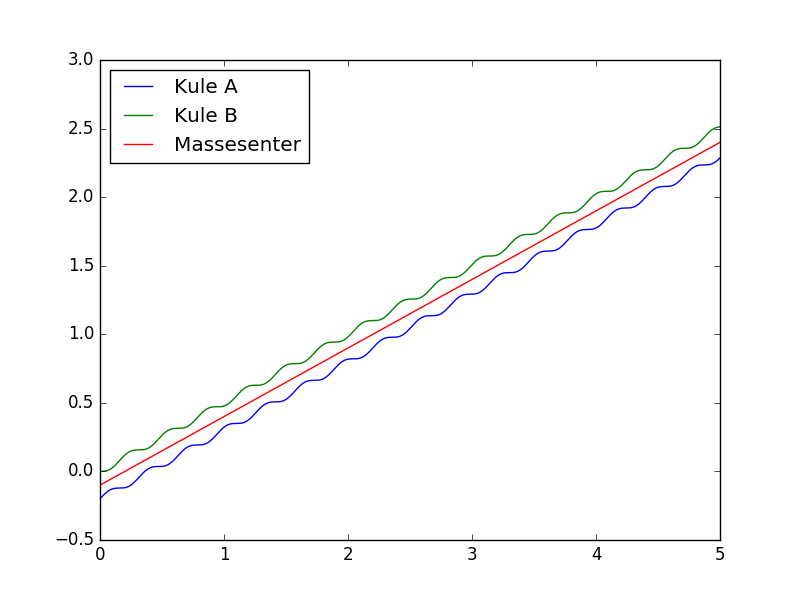
\includegraphics[width=12.6cm,height=8cm]{"C:/Users/Torstein/Documents/UiO/Fys-Mek1110/Python programmer"/Oblig6_h.png}
			\end{flushleft}












		\paragraph{i)}
			\begin{flushleft}
What is the maximum distance between the two atoms? \\
\vspace{1mm}
\textbf{Løsning:} \\
\vspace{1mm}
\lstinputlisting{oblig6_i.py}
Som vi ser blir den største avstanden $0.25$
			\end{flushleft}












		\paragraph{j)}
			\begin{flushleft}
What is the velocity of the center of mass and the angular velocity around the center of mass immediately after the collision? \\
\vspace{1mm}
\textbf{Løsning:} \\
\vspace{1mm}
				\begin{align}
P_0 = P_1 \nonumber \\
MV_0 = MV_1 \Rightarrow V_1 = \frac{1}{2}v_0 \nonumber \\
v_1 = \frac{1}{2}v_0 \nonumber \\
\omega = \frac{v}{R} = \frac{2v_0}{2b} = \frac{v_0}{b} \nonumber
				\end{align}
Der $v$ er farten til kule $A$ og  $V$ er farten til massesenteret, og $0$ og $1$ er før og etter kollisjonen.
			\end{flushleft}









		\paragraph{k)}
			\begin{flushleft}
Rewrite your program to model the motion of the atoms in this case. \\
\vspace{1mm}
\textbf{Løsning:} \\
\vspace{1mm}
\lstinputlisting{oblig6_k.py}
			\end{flushleft}










		\paragraph{l)}
			\begin{flushleft}
Plot the motion of the atoms and the center of mass after the collision. \\
\vspace{1mm}
\textbf{Løsning:} \\
\vspace{1mm}
\lstinputlisting{oblig6_l.py}
\includegraphics[width=12.6cm,height=8cm]{"C:/Users/Torstein/Documents/UiO/Fys-Mek1110/Python programmer"/Oblig6_l.png}
			\end{flushleft}








		\paragraph{m)}
			\begin{flushleft}
Discuss the motion of the angular velocity for the rotation about the center of mass for the motion after the collision. \\
\vspace{1mm}
\textbf{Løsning:} \\
\vspace{1mm}
Vinkelfarten vil øke når hver av kulene er på vei oppover i y retning og motsatt når de er på vei nedover i y retning.
			\end{flushleft}
\end{document}